\documentclass{article}

\usepackage{listings}[language=Python]
\usepackage{amsmath}
\usepackage{amssymb}
\usepackage{geometry}
\usepackage{fancyhdr}
\usepackage{graphicx}
\usepackage{array}
\usepackage{multirow}
\usepackage{tikz}
\usepackage{booktabs}
\usepackage{float}
\usepackage{xcolor}
\usetikzlibrary{calc,patterns,angles,quotes}

% for custom subsection
\usepackage{titlesec}
% package for enumerate with letters
\usepackage{enumitem}

\definecolor{codegreen}{rgb}{0,0.5,0}
\definecolor{codegray}{rgb}{0.4,0.4,0.4}
\definecolor{codepurple}{rgb}{0.5,0,0.5}
\definecolor{backcolour}{rgb}{0.9,0.9,0.9}
\definecolor{CornflowerBlue}{rgb}{0.6, 0.8, 1.0}

\lstdefinestyle{mystyle}{
    backgroundcolor=\color{backcolour},   
    commentstyle=\color{codegreen},
    keywordstyle=\color{red},
    numberstyle=\tiny\color{codegray},
    stringstyle=\color{codepurple},
    basicstyle=\ttfamily\footnotesize,
    breakatwhitespace=false,         
    breaklines=true,                 
    captionpos=b,                    
    keepspaces=true,                 
    numbers=left,                    
    numbersep=5pt,                  
    showspaces=false,                
    showstringspaces=false,
    showtabs=false,                  
    tabsize=2
}

\lstset{style=mystyle}

\titleformat{\subsection}
  {\normalfont\fontfamily{phv}\fontsize{14}{17}}{\thesubsection}{1em}{}

\newcommand\answer[1]{\colorbox{CornflowerBlue}{$#1$}}
\definecolor{CornflowerBlue}{rgb}{0.6, 0.8, 1.0}


\geometry{margin=1in}
\pagestyle{fancy}
\fancyhf{}
\rhead{Kyle Wodehouse}
\lhead{MSEG201}
\chead{Homework 4}
\title{\bfseries Homework 4}
\author{Kyle Wodehouse}
\rfoot{\thepage}
% 1 -> 5 from least to most descriptive
\setcounter{tocdepth}{1}

\begin{document}
\maketitle

\section{Polymer Structure}

\subsection*{a. polystyrene} 

% (i) Is the polymer a thermoplastic or thermoset?
% (ii) Determine a common object made from that polymer.
% (iii) Sketch the repeat unit.
% (iv) Determine the repeat unit molecular weight

(i) Polystyrene is a thermoplastic polymer. \\
(ii) A common object made from polystyrene is a styrofoam cup. \\
(iii) The repeat unit for polystyrene is shown below. 

\begin{figure}[H]
    \centering
    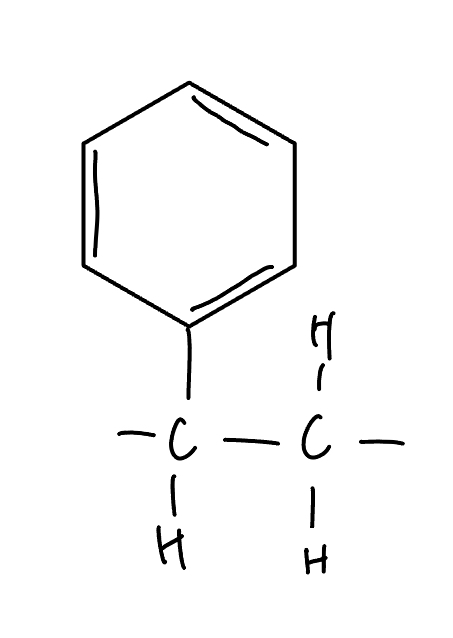
\includegraphics[width=0.3\textwidth]{polystyrene.jpeg}
\end{figure}

(iv) The repeat unit molecular weight is 104.15 g/mol.

\subsection*{b. polytetrafluoroethylene}

(i) Polytetrafluoroethylene is a thermoplastic polymer. \\
(ii) A common object made from polytetrafluoroethylene is teflon tape and non-stick cookware. \\
(iii) The repeat unit for polytetrafluoroethylene is shown below.

\begin{figure}[H]
    \centering
    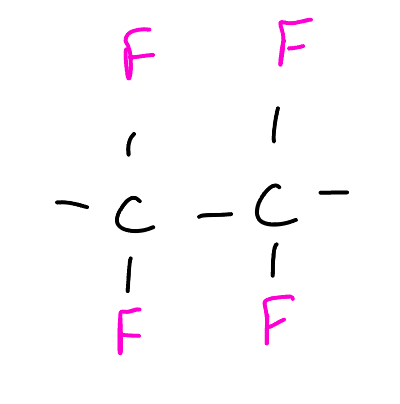
\includegraphics[width=0.3\textwidth]{ptfe.jpeg}
\end{figure}

(iv) The repeat unit molecular weight is 100.02 g/mol.

\subsection*{c. polydimethylsiloxane}

(i) Polydimethylsiloxane is a thermoplastic polymer. \\
(ii) A common object made from polydimethylsiloxane is silicone rubber. \\
(iii) The repeat unit for polydimethylsiloxane is shown below.

\begin{figure}[H]
    \centering
    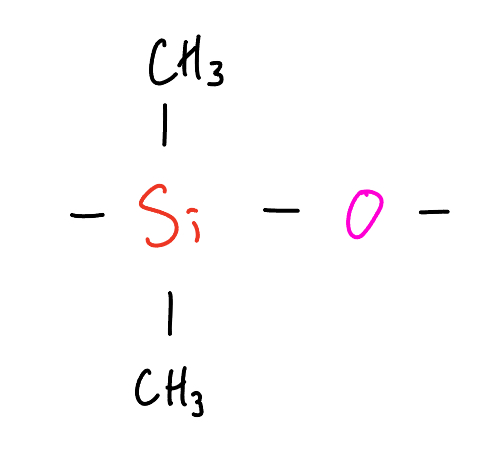
\includegraphics[width=0.3\textwidth]{pdms.jpeg}
\end{figure}
\noindent

(iv) The repeat unit molecular weight is 74.15 g/mol.


\subsection*{d. poly(methyl methacrylate)}

(i) Poly(methyl methacrylate) is a thermoplastic polymer. \\
(ii) A common object made from poly(methyl methacrylate) is plexiglass. \\
(iii) The repeat unit for poly(methyl methacrylate) is shown below.

\begin{figure}[H]
    \centering
    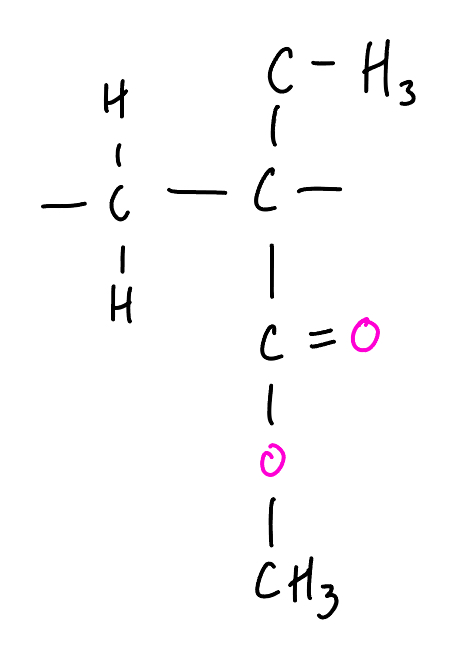
\includegraphics[width=0.3\textwidth]{pmma.jpeg}
\end{figure}

(iv) The repeat unit molecular weight is 100.12 g/mol.

\section{Polymer Molecular Weight}

For this question I could have used excel but I did it all in a jupter notebook (python) and then copied the code here. I hope this is okay since Prof. Hewlett did not explicitly say that this was okay, but he did say Excel is okay. The code is shown below

\begin{lstlisting}[language=Python]
    import numpy as np
    import matplotlib.pyplot as plt

    amounts = np.ones(4)
    molecular_weights = np.array([1e3,1e4,1e5,1e6])
    repeat_unit_weight = 104.15

    num_molecules =  amounts / molecular_weights

    mole_fractions = num_molecules / np.sum(num_molecules)
    number_average = np.sum(molecular_weights * mole_fractions)
    print(f'number average molecular weight: {number_average:.1f}')

    weight_fractions = amounts / np.sum(amounts)
    weight_average = np.sum(weight_fractions * molecular_weights) 
    print(f'weight average molecular weight: {weight_average}')

    ndegree_of_polymerization = number_average / repeat_unit_weight
    print(f'number average degree of polymerization: {ndegree_of_polymerization:.1f}')

    wdegree_of_polymerization = weight_average / repeat_unit_weight
    print(f'weight average degree of polymerization: {wdegree_of_polymerization:.1f}')

    pdi = weight_average / number_average
    print(f'polydispersity index: {pdi:.1f}')
\end{lstlisting}
\begin{table}[H]
    \centering
    \begin{tabular}{cc}
        \toprule
        \textbf{Property} & \textbf{Value} \\
        \midrule
        Number average molecular weight & 3600.4 \\
        Weight average molecular weight & 277750.0 \\
        Number average degree of polymerization & 34.6 \\
        Weight average degree of polymerization & 2666.8 \\
        Polydispersity index & 77.1 \\
        \bottomrule
    \end{tabular}
    \label{tab:polymer_molecular_weight}
\end{table}

\section{co-polymers}
\indent

I'll assume 100g as a basis for calculations to make my life easier

\[ 30\text{g Acrylonitrile} \times \frac{1 \text{mol}}{53.06 \text{g}} = 0.5654 \text{mol} \]
\[ 70\text{g Styrene (repeat units)} \times \frac{1 \text{mol}}{104.15 \text{g}} = 0.6721 \text{mol} \]

Now for the repeat unit aka mole fractions, denoted as $\chi$

\[ \chi_{\text{acrylonitrile}} = \frac{0.5654}{0.5654 + 0.6721} = \answer{0.4569} \]
\[ \chi_{\text{styrene}} = \frac{0.6721}{0.5654 + 0.6721} = \answer{0.5431} \]

\section{Crystallinity in Polymers}
\indent

Setting up the two equations

\[ 0.74 = \frac{\rho_c \left( 1.41 \text{g/cm}^3 - \rho_a \right)}{1.41 \text{g/cm}^3 \left( \rho_c - \rho_a \right)} \]

\[ 0.31 = \frac{\rho_c \left( 1.34 \text{g/cm}^3 - \rho_a \right)}{1.34 \text{g/cm}^3 \left( \rho_c - \rho_a \right)} \]

Which is a silly little system of equations. I'll isolate $\rho_c$ in the top equation

\[ \rho_c = \frac{\left(0.74 \cdot 1.41 \text{g/cm}^3\right) \cdot \rho_a}{\left(0.74 \cdot 1.41 \text{g/cm}^3 - 1.41 \text{g/cm}^3\right) + \rho_a} = \frac{1.043 \rho_a}{\rho_a - 0.367} \]

Now taking that and plugging it back into the second equation

\[ 0.31 = \frac{\rho_c \left( 1.34 \text{g/cm}^3 - \rho_a \right)}{1.34 \text{g/cm}^3 \left( \rho_c - \rho_a \right)} = \frac{\frac{1.043 \rho_a}{\rho_a - 0.367} \left( 1.34 \text{g/cm}^3 - \rho_a \right)}{1.34 \text{g/cm}^3 \left( \frac{1.043 \rho_a}{\rho_a - 0.367} - \rho_a \right)} \]

In theory this could be solved by hand, but\dots I just plugged it into wolfram alpha and got this solution

\[ \rho_a = \answer{1.29 \text{g/cm}^3} \]

and then since I have $\rho_a$ I can plug it back into the equation for $\rho_c$

\[ \rho_c = \frac{1.043 \cdot 1.29}{1.29 - 0.367} = \answer{1.46 \text{g/cm}^3} \]

\subsection*{b.}
\indent

Bringing back the original formula for the degree of Crystallinity

\[ \chi_s = \frac{\rho_c \left( \rho_s - \rho_a \right)}{\rho_s \left( \rho_c - \rho_a \right)} \]

Now just plugging in the known densities and the new 1.38 sample density

\[ \chi_s = \frac{1.46 \cdot \left( 1.38 - 1.29 \right)}{1.38 \cdot \left( 1.46 - 1.29 \right)} = \answer{0.56} \]

As an interesting side note I wanted to plot the volume of a sample as a function fo the degree of crystallinity. I used the following formula

\[ \rho_s = \frac{\rho_c \rho_a}{\rho_c + \chi_s \rho_a - \chi_s \rho_c} \]

Which looks like

\begin{figure}[H]
    \centering
    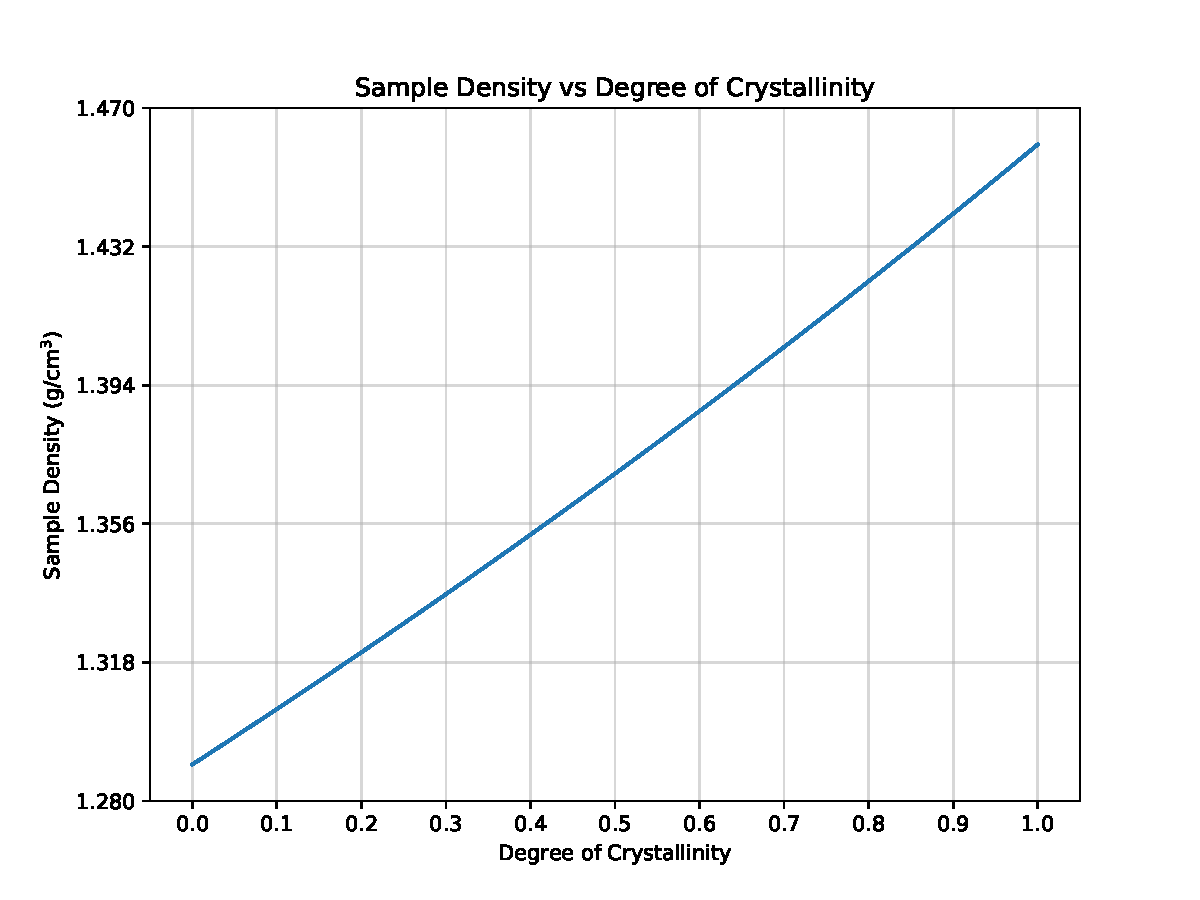
\includegraphics[width=0.95\textwidth]{density_vs_crystallinity.pdf}
\end{figure}

This is actually quite an interesting trend. As the degree of crystallinity increases the density of the sample increases, but not linearly. Very cool.




\end{document}